\documentclass[12pt]{article}
\usepackage{amsmath}
\usepackage{graphicx}
\usepackage{hyperref}
\usepackage{listings}
\usepackage{color}
\usepackage{pythonhighlight}

\title{Operating System Course Report - First Half of the Semester}
\author{A class}
\date{\today}

\begin{document}

\maketitle
\newpage

\tableofcontents
\newpage

\section{Introduction}
This report summarizes the topics covered during the first half of the Operating System course. It includes theoretical concepts, practical implementations, and assignments. The course focuses on the fundamentals of operating systems, including system architecture, process management, CPU scheduling, and deadlock handling.

\section{Course Overview}
\subsection{Objectives}
The main objectives of this course are:
\begin{itemize}
    \item To understand the basic components and architecture of a computer system.
    \item To learn process management, scheduling, and inter-process communication.
    \item To explore file systems, input/output management, and virtualization.
    \item To study the prevention and handling of deadlocks in operating systems.
\end{itemize}

\subsection{Course Structure}
The course is divided into two halves. This report focuses on the first half, which covers:
\begin{itemize}
    \item Basic Concepts and Components of Computer Systems
    \item System Performance and Metrics
    \item System Architecture of Computer Systems
    \item Process Description and Control
    \item Scheduling Algorithms
    \item Process Creation and Termination
    \item Introduction to Threads
    \item File Systems
    \item Input and Output Management
    \item Deadlock Introduction and Prevention
    \item User Interface Management
    \item Virtualization in Operating Systems
\end{itemize}

\section{Topics Covered}

\subsection{Basic Concepts and Components of Computer Systems}
This section explains the fundamental components that make up a computer system, including the CPU, memory, storage, and input/output devices.

\subsection{System Performance and Metrics}
This section introduces various system performance metrics used to measure the efficiency of a computer system, including throughput, response time, and utilization.

\subsection{System Architecture of Computer Systems}
Describes the architecture of modern computer systems, focusing on the interaction between hardware and the operating system.

\subsection{Process Description and Control}
Processes are a central concept in operating systems. This section covers:
\begin{itemize}
    \item Process states and state transitions
    \item Process control block (PCB)
    \item Context switching
\end{itemize}

\subsection{Scheduling Algorithms}
This section covers:
\begin{itemize}
    \item First-Come, First-Served (FCFS)
    \item Shortest Job Next (SJN)
    \item Round Robin (RR)
\end{itemize}
It explains how these algorithms are used to allocate CPU time to processes.

\subsection{Process Creation and Termination}
Details how processes are created and terminated by the operating system, including:
\begin{itemize}
    \item Process spawning
    \item Process termination conditions
\end{itemize}

\subsection{Introduction to Threads}
This section introduces the concept of threads and their relation to processes, covering:
\begin{itemize}
    \item Single-threaded vs. multi-threaded processes
    \item Benefits of multithreading
\end{itemize}

\begin{figure}[h]
    \centering
    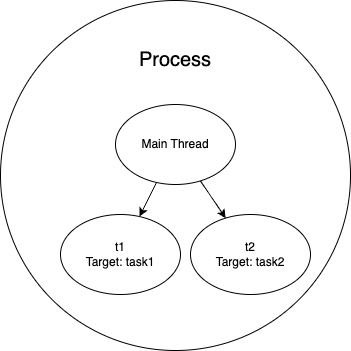
\includegraphics[width=0.5\textwidth]{asset/example.png}  % Sesuaikan nama file dan ukurannya
    \caption{Ini adalah gambar contoh dari multithreading.}
    \label{fig:contoh_gambar}
\end{figure}

Seperti yang terlihat pada Gambar \ref{fig:contoh_gambar}, inilah cara menambahkan gambar dengan keterangan.

\subsection{File Systems}
File systems provide a way for the operating system to store, retrieve, and manage data. This section explains:
\begin{itemize}
    \item File system structure
    \item File access methods
    \item Directory management
\end{itemize}

\subsection{Input and Output Management}
Input and output management is key for handling the interaction between the system and external devices. This section includes:
\begin{itemize}
    \item Device drivers
    \item I/O scheduling
\end{itemize}

\subsection{Deadlock Introduction and Prevention}

Explores the concept of deadlocks and methods for preventing them:
\begin{itemize}
    \item[]
\end{itemize}

\subsubsection{Deadlock Conditions}

\subsubsection{Pencegahan Terhadap Deadlock}
\textbf{3.10.2.3   Kelebihan dan Kekurangan dari Pencegahan Deadlock\\}

\textbf{1. Resource Allocation Denial\\}

    Kelebihan dari pencegahan ini, yaitu :\\

    a.	Menjamin bahwa sistem tidak akan masuk ke keadaan deadlock

    Dengan menggunakan metode ini, sistem memastikan bahwa tidak ada proses yang diberikan sumber daya jika pengalokasian tersebut berpotensi menyebabkan deadlock. Artinya, sebelum sumber daya dialokasikan, sistem melakukan pengecekan apakah alokasi tersebut aman atau tidak. Hal ini sangat penting terutama untuk sistem kritis dimana downtime akibat deadlock bisa mengakibatkan kerugian besar atau risiko keamanan tinggi.\\

    b.	Algoritma Banker's memberikan solusi optimal dalam pengalokasian sumber daya
    
    Algoritma Banker's bekerja dengan memperhitungkan kebutuhan maksimum dari setiap proses dan hanya mengalokasikan sumber daya jika sistem tetap berada dalam keadaan aman. Ini menjamin bahwa semua proses dapat menyelesaikan eksekusinya tanpa menunggu sumber daya secara terus-menerus, sehingga mengoptimalkan penggunaan sumber daya yang ada di sistem.\\

    c.	Cocok untuk sistem yang memprioritaskan kestabilan dan keamanan pengelolaan sumber daya
    
    Sistem yang sangat sensitif terhadap kegagalan atau memiliki risiko tinggi jika terjadi deadlock akan sangat diuntungkan dengan pendekatan ini. Metode ini memberikan keamanan tambahan karena setiap pengalokasian dipastikan aman, menjadikannya sangat ideal untuk sistem seperti layanan kesehatan atau sistem keuangan.\\

    d.	Mengurangi risiko kelambatan atau deadlock pada sistem yang membutuhkan kontrol ketat
    
    Dalam sistem dimana sumber daya terbatas dan pengelolaannya membutuhkan kontrol ketat, metode ini bisa mengurangi kemungkinan proses berhenti akibat deadlock. Hal ini karena semua pengalokasian sumber daya dilakukan hanya jika sudah diverifikasi aman, sehingga proses bisa berjalan lebih lancar tanpa gangguan yang disebabkan oleh deadlock.\\
    
    Kekurangan dari pencegahan ini, yaitu:\\

	a. Overhead komputasi tinggi

    Kelemahan terbesar dari metode ini adalah kebutuhan akan sumber daya komputasi yang signifikan untuk memeriksa apakah setiap alokasi aman. Sistem harus menghitung ulang setiap kali ada permintaan sumber daya baru, yang bisa memakan waktu dan mempengaruhi performa, terutama pada sistem yang memiliki banyak proses dan sumber daya.\\

	b. Tidak praktis untuk sistem besar dengan banyak proses dan sumber daya

    Untuk sistem yang melibatkan banyak proses dan sumber daya yang saling bersaing, metode ini menjadi sangat tidak praktis. Setiap kali proses meminta sumber daya, sistem harus mengecek keadaan aman, yang menyebabkan overhead besar. Dalam sistem besar, ini bisa memperlambat kinerja dan menambah kompleksitas.\\

	c. Memerlukan informasi lengkap tentang jumlah sumber daya yang dibutuhkan setiap proses, yang bisa sulit diestimasi

    Algoritma ini membutuhkan informasi lengkap mengenai kebutuhan maksimum dari setiap proses. Namun, dalam praktiknya, seringkali sulit atau tidak mungkin untuk memprediksi dengan akurat berapa jumlah sumber daya yang benar-benar dibutuhkan oleh setiap proses, terutama pada sistem dinamis dimana kebutuhan bisa berubah-ubah.\\

	d. Tidak fleksibel

    Metode ini kurang fleksibel dalam menghadapi perubahan. Jika ada sedikit perubahan dalam kebutuhan sumber daya proses, sistem mungkin menolak pengalokasian karena dianggap tidak aman. Hal ini bisa membuat beberapa proses ditolak secara berlebihan, meskipun sebenarnya mereka hanya membutuhkan sedikit penyesuaian alokasi.\\

\textbf{2. Resource Ordering\\}

    Kelebihan dari pencegahan ini, yaitu :\\

    a. Sederhana dan efektif dalam mencegah deadlock
    
    Salah satu kelebihan terbesar dari metode ini adalah kesederhanaannya. Dengan menetapkan urutan tertentu dalam pengalokasian sumber daya, sistem bisa mencegah deadlock tanpa memerlukan algoritma yang rumit. Setiap proses harus meminta sumber daya sesuai urutan yang sudah ditentukan, sehingga menghindari potensi deadlock yang bisa terjadi jika proses meminta sumber daya dalam urutan acak.\\

    b. Tidak memerlukan pengecekan kondisi sistem seperti metode avoidance (penghindaran)
    
    Berbeda dengan metode yang lebih kompleks seperti avoidance, resource ordering tidak memerlukan pengecekan terus-menerus terhadap kondisi sistem. Ini membuat metode ini lebih ringan secara komputasi, karena sistem tidak perlu menghitung apakah alokasi sumber daya aman atau tidak sebelum melakukan pengalokasian.\\

    c. Meminimalkan kebutuhan pengawasan sumber daya secara dinamis, sehingga mengurangi overhead pada sistem
    
    Karena sumber daya dialokasikan berdasarkan urutan tetap, tidak ada kebutuhan untuk melakukan pengawasan terus-menerus terhadap status sumber daya atau proses. Ini mengurangi overhead yang biasanya terjadi pada metode yang lebih kompleks, dimana sistem harus memantau pengalokasian sumber daya secara dinamis.\\

    d. Sederhana untuk diimplementasikan dalam sistem dengan sedikit sumber daya
    
    Dalam sistem yang memiliki sedikit jenis sumber daya, metode ini sangat efektif. Implementasinya tidak memerlukan kompleksitas tambahan karena jumlah sumber daya yang terbatas mempermudah pengelolaan dan penetapan urutan alokasi. Sistem bisa berjalan dengan lancar karena urutan alokasi mudah diatur.\\

    Kekurangan dari pencegahan ini, yaitu :\\

    a. Membatasi fleksibilitas proses dalam meminta sumber daya
    
    Dengan adanya urutan tetap dalam permintaan sumber daya, proses tidak bisa dengan bebas meminta sumber daya sesuai kebutuhan mereka secara dinamis. Ini bisa membatasi fleksibilitas proses, terutama jika kebutuhan sumber daya berubah di tengah jalan, yang membuat mereka harus menunggu lebih lama.\\

    b. Tidak selalu efisien
    
    Salah satu kekurangan utama dari metode ini adalah kurangnya efisiensi dalam beberapa situasi. Jika satu proses memerlukan banyak sumber daya tetapi harus mengikuti urutan yang ditetapkan, proses tersebut mungkin harus menunggu lebih lama dibandingkan dengan metode lain yang lebih fleksibel.\\

    c. Tidak skalabel dalam sistem yang lebih kompleks dengan banyak jenis sumber daya
    
    Metode ini kurang cocok untuk sistem yang lebih besar dan lebih kompleks dimana ada banyak jenis sumber daya yang berbeda. Mengatur urutan tetap untuk banyak sumber daya bisa menjadi sangat rumit dan tidak efisien, sehingga metode ini tidak efektif untuk sistem besar dengan berbagai kebutuhan.\\

    d. Pengurutan sumber daya statis mungkin tidak efektif jika pola penggunaan sumber daya berubah secara dinamis
    
    Jika pola penggunaan sumber daya di sistem berubah secara dinamis, metode ini bisa menjadi tidak efektif. Urutan yang ditetapkan sebelumnya mungkin tidak relevan dengan pola penggunaan baru, menyebabkan sistem menjadi kurang efisien atau bahkan rentan terhadap deadlock jika urutan tidak bisa diikuti.\\

\textbf{3. Avoidance of Hold-and-Wait Conditions\\}

    Kelebihan dari pencegahan ini, yaitu :\\

    a. Mencegah kondisi deadlock dengan menghilangkan salah satu dari empat kondisi deadlock (\textit{hold-and-wait})
    
    Metode ini mencegah deadlock dengan memastikan bahwa proses tidak akan memegang satu sumber daya sambil menunggu sumber daya lain. Semua sumber daya yang dibutuhkan oleh proses harus diminta sekaligus, sehingga menghindari situasi dimana satu proses menunggu sumber daya yang sedang dipegang oleh proses lain. Ini adalah pendekatan preventif yang sangat efektif dalam menghilangkan salah satu syarat terjadinya deadlock.\\

    b. Lebih mudah diterapkan dalam beberapa sistem kecil atau dengan sumber daya terbatas
    
    Dalam sistem yang memiliki jumlah sumber daya terbatas dan sedikit proses, pendekatan ini relatif mudah diterapkan. Karena jumlah proses dan sumber daya yang harus diawasi lebih sedikit, aturan untuk meminta semua sumber daya sekaligus dapat diterapkan dengan lebih mudah, tanpa menimbulkan banyak overhead atau beban pada sistem.\\

    c. Mengurangi kompleksitas dalam sistem yang memerlukan manajemen sumber daya yang sederhana
    
    Sistem yang sederhana atau dengan pola penggunaan sumber daya yang tetap dapat memanfaatkan metode ini untuk mengurangi kompleksitas manajemen sumber daya. Tidak ada kebutuhan untuk melakukan pengecekan yang rumit atau algoritma yang kompleks, karena semua permintaan sumber daya dikelola secara bersamaan.\\

    d. Meningkatkan transparansi alokasi sumber daya karena semua sumber daya diminta sekaligus
    
    Dengan proses yang meminta semua sumber daya yang dibutuhkan di awal, transparansi alokasi meningkat. Administrator sistem dapat lebih mudah memonitor kebutuhan proses dan mencegah potensi konflik alokasi di masa depan. Ini juga membantu dalam merencanakan dan mengelola sumber daya secara lebih efektif.\\

    Kekurangan dari pencegahan ini, yaitu :\\

    a. Mungkin menghasilkan inefisiensi, karena proses harus menunggu lebih lama untuk mendapatkan semua sumber daya yang diperlukan
    
    Salah satu kekurangan terbesar dari pendekatan ini adalah bahwa proses harus menunggu hingga semua sumber daya yang diperlukan tersedia sebelum dapat memulai. Jika salah satu sumber daya tidak tersedia, proses harus menunggu, yang bisa mengakibatkan penurunan efisiensi karena sumber daya yang lain sudah tersedia namun tidak digunakan.\\

    b. Pemborosan sumber daya karena proses mungkin memegang sumber daya yang tidak segera digunakan
    
    Karena semua sumber daya diminta sekaligus, ada kemungkinan beberapa sumber daya yang dialokasikan tidak langsung digunakan. Hal ini bisa menyebabkan pemborosan, dimana sumber daya yang sudah dialokasikan tidak dimanfaatkan dengan baik, sementara proses lain yang membutuhkan sumber daya tersebut harus menunggu.\\

    c. Membatasi multitasking karena proses harus menunggu sampai semua sumber daya tersedia
    
    Proses tidak dapat mulai menjalankan sebagian tugasnya sambil menunggu sisa sumber daya yang diperlukan. Ini membatasi kemampuan sistem untuk melakukan multitasking atau menjalankan beberapa proses secara bersamaan, karena setiap proses harus menunggu sampai semua sumber daya yang dibutuhkan tersedia.\\

    d. Dalam kasus tertentu, bisa menyebabkan starvation (proses terus-menerus gagal mendapatkan sumber daya karena harus menunggu lama)
    
    Jika ada proses yang membutuhkan banyak sumber daya, terutama di lingkungan dengan sumber daya terbatas, proses tersebut bisa mengalami starvation. Artinya, proses mungkin terus menunggu sumber daya yang tidak pernah tersedia karena dialokasikan ke proses lain, menyebabkan penundaan yang berkepanjangan. \\

\textbf{4. Timeout\\}

    Kelebihan dari pencegahan ini, yaitu :\\

    a. Mudah diimplementasikan dan tidak memerlukan pengaturan kompleks
    
    Metode ini sangat sederhana dan mudah untuk diimplementasikan karena hanya memerlukan penetapan batas waktu untuk setiap proses yang sedang menunggu sumber daya. Jika batas waktu tersebut terlewati, proses akan dihentikan atau di-reset. Pendekatan ini tidak memerlukan algoritma rumit atau pengawasan kompleks, sehingga dapat diterapkan pada banyak jenis sistem tanpa membutuhkan modifikasi besar.\\

    b. Memberikan jaminan bahwa proses tidak akan menunggu sumber daya selamanya 
    
    Salah satu kelebihan utama dari metode timeout adalah bahwa ia memberikan jaminan bahwa proses tidak akan terjebak menunggu sumber daya tanpa batas waktu. Jika sumber daya yang diperlukan tidak tersedia dalam jangka waktu tertentu, proses akan dihentikan atau di-reset, memberikan kesempatan bagi proses lain untuk mendapatkan akses ke sumber daya tersebut.\\

    c. Mengoptimalkan waktu proses yang terjebak dalam antrian sumber daya dengan memberikan kesempatan pada proses lain untuk berjalan
    
    Dengan adanya batas waktu, proses yang terlalu lama menunggu sumber daya akan dihentikan atau dialihkan, sehingga menghindari bottleneck di sistem. Proses lain yang mungkin bisa berjalan dengan sumber daya yang tersedia dapat mulai berjalan lebih cepat, meningkatkan efisiensi sistem secara keseluruhan.\\

    d. Memungkinkan sistem tetap responsif dalam menghadapi deadlock sementara
    
    Jika terjadi deadlock sementara  beberapa proses saling menunggu sumber daya, metode timeout dapat membantu memutus lingkaran deadlock tersebut. Ketika salah satu proses mencapai batas waktunya dan dihentikan, sumber daya yang terlibat dalam deadlock bisa dilepaskan, memungkinkan proses lain untuk melanjutkan eksekusi dan sistem tetap responsif.\\

    Kekurangan dari pencegahan ini, yaitu :\\

    a. Tidak menjamin bahwa deadlock benar-benar dihindari, hanya meresolusi setelah terjadi
    
    Salah satu kelemahan utama dari metode ini adalah bahwa deadlock tidak dicegah sejak awal. Proses bisa tetap terjebak dalam deadlock untuk sementara waktu sampai batas waktu tercapai. Metode ini lebih berfungsi sebagai solusi setelah deadlock terjadi, bukan sebagai pencegahan deadlock.\\

    b. Proses mungkin harus dimulai ulang jika timeout, yang bisa menjadi inefisien dan menyebabkan penurunan kinerja sistem
    
    Jika proses dihentikan karena timeout, ada kemungkinan besar bahwa proses tersebut harus dimulai ulang dari awal, terutama jika sumber daya yang dibutuhkan masih belum tersedia. Hal ini dapat menyebabkan penurunan kinerja sistem karena waktu dan sumber daya yang sudah digunakan untuk proses tersebut terbuang sia-sia.\\

    c. Menambah overhead untuk memonitor batas waktu pada setiap proses
    
    Sistem harus terus memonitor waktu yang dihabiskan oleh setiap proses untuk memastikan apakah batas waktu sudah tercapai atau belum. Ini menambah overhead pada sistem, terutama jika ada banyak proses yang harus dipantau secara bersamaan, dan bisa mempengaruhi efisiensi keseluruhan sistem.\\

    d. Batas waktu yang tidak tepat dapat menyebabkan proses yang memerlukan sumber daya besar mengalami kegagalan berulang
    
    Jika batas waktu yang ditetapkan terlalu singkat, proses yang memerlukan banyak sumber daya mungkin tidak pernah mendapatkan cukup waktu untuk menyelesaikan tugasnya, dan terus menerus dihentikan. Ini bisa menyebabkan kegagalan berulang, dimana proses besar tidak pernah selesai, mempengaruhi kinerja sistem secara keseluruhan.\\

    \begin{thebibliography}{9}

        \bibitem{silberschatz2018} 
        Silberschatz, A., Galvin, P. B., \& Gagne, G. (2018). \textit{Operating system concepts} (10th ed.). Wiley.
        
        \bibitem{stallings2018} 
        Stallings, W. (2018). \textit{Operating systems: Internals and design principles} (9th ed.). Pearson.
        
        \bibitem{tanenbaum2014} 
        Tanenbaum, A. S., \& Bos, H. (2014). \textit{Modern operating systems} (4th ed.). Pearson.
        
    \end{thebibliography}

\subsection{User Interface Management}
This section discusses the role of the operating system in managing the user interface. Topics covered include:
\begin{itemize}
    \item Graphical User Interface (GUI)
    \item Command-Line Interface (CLI)
    \item Interaction between the user and the operating system
\end{itemize}

\subsection{Virtualization in Operating Systems}

Virtualization allows multiple operating systems to run concurrently on a single physical machine. This section explores:
\begin{itemize}
    \item Concept of virtualization
    \item Hypervisors and their types
    \item Benefits of virtualization in modern computing
\end{itemize}

\section{Assignments and Practical Work}
\subsection{Assignment 1: Process Scheduling}
Students were tasked with implementing various process scheduling algorithms (e.g., FCFS, SJN, and RR) and comparing their performance under different conditions.
\subsubsection{Group 1}
\begin{python}
    class Process:
    def __init__(self, pid, arrival_time, burst_time):
        self.pid = pid
        self.arrival_time = arrival_time
        self.burst_time = burst_time
        self.completion_time = 0
        self.turnaround_time = 0
        self.waiting_time = 0
\end{python}

\begin{table}[htbp] % Optional: For floating position
    \centering
    \begin{tabular}{|c|c|c|} % Defines number of columns and alignment (c = center, l = left, r = right). '|' creates vertical lines.
    \hline
    Header 1 & Header 2 & Header 3 \\ % Column headers
    \hline
    Row 1, Column 1 & Row 1, Column 2 & Row 1, Column 3 \\ % First row of data
    \hline
    Row 2, Column 1 & Row 2, Column 2 & Row 2, Column 3 \\ % Second row of data
    \hline
    \end{tabular}
    \caption{Your table caption} % Optional: For adding a caption
    \label{tab:your_label} % Optional: For cross-referencing the table
\end{table}
\subsection{Assignment 2: Deadlock Handling}
In this assignment, students were asked to simulate different deadlock scenarios and explore various prevention methods.

\subsection{Assignment 3: Multithreading and Amdahl's Law}
This assignment involved designing a multithreading scenario to solve a computationally intensive problem. Students then applied **Amdahl's Law** to calculate the theoretical speedup of the program as the number of threads increased.

\subsection{Assignment 4: Simple Command-Line Interface (CLI) for User Interface Management}
Students were tasked with creating a simple **CLI** for user interface management. The CLI should support basic commands such as file manipulation (creating, listing, and deleting files), process management, and system status reporting.
\subsubsection{Group 11}

\textbf{Soal}\\
Andi bekerja sebagai seorang administrator sistem di sebuah perusahaan teknologi. Suatu hari, ia diminta oleh atasannya untuk membuat sebuah aplikasi sederhana berbasis Command-Line Interface (CLI) yang akan mempermudah timnya dalam mengelola proses yang berjalan di server.\\
\\
Aplikasi tersebut harus mampu melakukan hal-hal berikut:\\
\\
1.Melihat daftar proses yang sedang berjalan di server, termasuk menampilkan PID dan nama dari setiap proses.
\\
2.Menghentikan proses tertentu berdasarkan PID jika proses tersebut menyebabkan masalah.
\\
3.Menampilkan status sistem, seperti penggunaan CPU, memori, dan disk untuk memastikan server berjalan dalam kondisi optimal.\\
\\
Bantulah Andi dengan membuat aplikasi CLI menggunakan Python yang dapat menyelesaikan tiga tugas di atas!
\\
\textbf{Jawaban}\\
Untuk menyelesaikan masalah ini, kita akan menggunakan modul Python psutil untuk memantau proses dan status sistem, serta argparse untuk membuat interface command-line yang dapat menerima input dari pengguna.\\
\\
Sebelum masuk ke kode python, pertama kita buka terminal dan input kode ini :\\
\\
\begin{text}
    pip install psutil\\
\end{text}
\\
Berikut adalah solusi Python untuk masalah yang dihadapi Andi:
\begin{python}
    import psutil
    import argparse

    def list_processes():
        processes = psutil.pids()
        print(f"Daftar proses yang berjalan di sistem:")
        for pid in processes:
            try:
                process = psutil.Process(pid)
                print(f"PID: {pid}, Nama: {process.name()}")
            except psutil.NoSuchProcess:
                pass

    def kill_process(pid):
        try:
            process = psutil.Process(pid)
            process.terminate()
            print(f"Proses dengan PID {pid} berhasil dihentikan.")
        except psutil.NoSuchProcess:
            print(f"Tidak ada proses dengan PID {pid}.")
        except Exception as e:
            print(f"Gagal menghentikan proses: {e}")

    def system_status():
        print(f"Penggunaan CPU: {psutil.cpu_percent()}%")
        print(f"Penggunaan RAM: {psutil.virtual_memory().percent}%")
        print(f"Penggunaan Disk: {psutil.disk_usage('/').percent}%")

    if __name__ == "__main__":
        parser = argparse.ArgumentParser(description="CLI untuk manajemen proses dan status sistem")

        subparsers = parser.add_subparsers(dest='command')

        list_parser = subparsers.add_parser('list', help='Menampilkan daftar proses yang berjalan')

        kill_parser = subparsers.add_parser('kill', help='Menghentikan proses berdasarkan PID')
        kill_parser.add_argument('pid', type=int, help='PID dari proses yang akan dihentikan')

        status_parser = subparsers.add_parser('status', help='Menampilkan status sistem')

        args = parser.parse_args()

        if args.command == 'list':
            list_processes()
        elif args.command == 'kill':
            kill_process(args.pid)
        elif args.command == 'status':
            system_status()
\end{python}
Penjelasan:\\

1.Daftar Proses
\begin{itemize}
    \item Fungsi \texttt{list\_processes()} mengambil semua PID dari proses yang berjalan menggunakan \texttt{psutil.pids()}. Untuk setiap PID, kita membuat objek proses dengan \texttt{psutil.Process(pid)} dan menampilkan PID serta nama prosesnya.
\end{itemize}

2.Menghentikan Proses
\begin{itemize}
    \item Fungsi \texttt{kill\_process()} menerima PID dari proses yang ingin dihentikan. Proses dihentikan menggunakan \texttt{process.terminate()}. Jika PID tidak ditemukan, akan ada pesan kesalahan yang ditampilkan.
\end{itemize}

3. Status Sistem
\begin{itemize}
    \item Fungsi \texttt{system\_status()} menampilkan penggunaan CPU, RAM, dan disk menggunakan fungsi \texttt{psutil} yang relevan seperti \texttt{cpu\_percent()}, \texttt{virtual\_memory().percent}, dan \texttt{disk\_usage('/')}.\\\\\\\\
\end{itemize}
Andi dapat menjalankan aplikasi CLI ini di terminal dengan tiga perintah utama:\\
\\
1. Melihat Daftar Proses
\\
Untuk melihat daftar proses yang berjalan, Andi dapat menggunakan perintah berikut:\\

\begin{verbatim}
python cli.py list
\end{verbatim}
Ini akan menampilkan semua proses yang berjalan dengan PID dan nama prosesnya.\\
\\
2. Menghentikan Proses Berdasarkan PID\\
\\
Untuk menghentikan proses berdasarkan PID, Andi dapat menjalankan perintah berikut:
\\
\begin{verbatim}
python cli.py kill <PID>
\end{verbatim}
Sebagai contoh, untuk menghentikan proses dengan PID 1234, Andi dapat mengetik:\\
\begin{verbatim}
python cli.py kill 1234
\end{verbatim}
3. Melihat Status Sistem\\
\\
Untuk melihat status sistem seperti penggunaan CPU, RAM, dan disk, Andi dapat menjalankan perintah berikut:
\\
\begin{verbatim}
python cli.py status
\end{verbatim}
Ini akan menampilkan informasi mengenai penggunaan CPU, RAM, dan disk pada server.
\\
\subsection{Assignment 5: File System Access}
In this assignment, students implemented file system access routines, including:
\begin{itemize}
    \item File creation and deletion
    \item Reading from and writing to files
    \item Navigating directories and managing file permissions
\end{itemize}

\subsubsection{Group 11}

\textbf{Soal}
\\
Anita sedang bekerja di perusahaan teknologi dan diberikan tugas untuk membuat laporan penjualan dalam bentuk file teks. Laporan tersebut harus dibuat setiap minggu. Sebelum menulis laporan baru, Anita harus membuat file dengan nama "laporan\_penjualan\_mingguan.txt". Namun, saat ia mencoba membuat file, sistem menolak permintaan karena ada file dengan nama yang sama. Bagaimana Anita dapat menghapus file lama tersebut agar bisa membuat file yang baru?
\\\\
\textbf{Jawaban}\\
Anita dapat menghapus file lama dengan menggunakan modul Python os. Berikut adalah contoh kode Python yang bisa digunakan untuk menghapus file lama dan kemudian membuat file baru:\\
\begin{python}
    import os

    filename = "laporan_penjualan_mingguan.txt"

    if os.path.exists(filename):
        os.remove(filename)
        print(f"File '{filename}' berhasil dihapus.")
    else:
        print(f"File '{filename}' tidak ditemukan.")

    with open(filename, "w") as file:
        file.write("Ini adalah laporan penjualan mingguan yang baru.")
        print(f"File '{filename}' berhasil dibuat dan diisi dengan laporan baru.")

\end{python}
Penjelasan untuk kode diatas:
\\
1. os.path.exists() digunakan untuk memeriksa apakah file dengan nama yang sama sudah ada.\\
2. Jika file sudah ada, maka os.remove() digunakan untuk menghapus file tersebut.\\
3.Setelah file lama dihapus, kita membuat file baru menggunakan open() dengan mode "w" untuk menulis laporan baru ke dalam file.\\
\section{Conclusion}
The first half of the course introduced core operating system concepts, including process management, scheduling, multithreading, and file system access. These topics provided a foundation for more advanced topics to be covered in the second half of the course.

\end{document}